% Options for packages loaded elsewhere
% Options for packages loaded elsewhere
\PassOptionsToPackage{unicode}{hyperref}
\PassOptionsToPackage{hyphens}{url}
\PassOptionsToPackage{dvipsnames,svgnames,x11names}{xcolor}
%
\documentclass[
  11pt,
]{article}
\usepackage{xcolor}
\usepackage[margin=1in]{geometry}
\usepackage{amsmath,amssymb}
\setcounter{secnumdepth}{5}
\usepackage{iftex}
\ifPDFTeX
  \usepackage[T1]{fontenc}
  \usepackage[utf8]{inputenc}
  \usepackage{textcomp} % provide euro and other symbols
\else % if luatex or xetex
  \usepackage{unicode-math} % this also loads fontspec
  \defaultfontfeatures{Scale=MatchLowercase}
  \defaultfontfeatures[\rmfamily]{Ligatures=TeX,Scale=1}
\fi
\usepackage{lmodern}
\ifPDFTeX\else
  % xetex/luatex font selection
\fi
% Use upquote if available, for straight quotes in verbatim environments
\IfFileExists{upquote.sty}{\usepackage{upquote}}{}
\IfFileExists{microtype.sty}{% use microtype if available
  \usepackage[]{microtype}
  \UseMicrotypeSet[protrusion]{basicmath} % disable protrusion for tt fonts
}{}
\usepackage{setspace}
\makeatletter
\@ifundefined{KOMAClassName}{% if non-KOMA class
  \IfFileExists{parskip.sty}{%
    \usepackage{parskip}
  }{% else
    \setlength{\parindent}{0pt}
    \setlength{\parskip}{6pt plus 2pt minus 1pt}}
}{% if KOMA class
  \KOMAoptions{parskip=half}}
\makeatother
% Make \paragraph and \subparagraph free-standing
\makeatletter
\ifx\paragraph\undefined\else
  \let\oldparagraph\paragraph
  \renewcommand{\paragraph}{
    \@ifstar
      \xxxParagraphStar
      \xxxParagraphNoStar
  }
  \newcommand{\xxxParagraphStar}[1]{\oldparagraph*{#1}\mbox{}}
  \newcommand{\xxxParagraphNoStar}[1]{\oldparagraph{#1}\mbox{}}
\fi
\ifx\subparagraph\undefined\else
  \let\oldsubparagraph\subparagraph
  \renewcommand{\subparagraph}{
    \@ifstar
      \xxxSubParagraphStar
      \xxxSubParagraphNoStar
  }
  \newcommand{\xxxSubParagraphStar}[1]{\oldsubparagraph*{#1}\mbox{}}
  \newcommand{\xxxSubParagraphNoStar}[1]{\oldsubparagraph{#1}\mbox{}}
\fi
\makeatother


\usepackage{longtable,booktabs,array}
\usepackage{calc} % for calculating minipage widths
% Correct order of tables after \paragraph or \subparagraph
\usepackage{etoolbox}
\makeatletter
\patchcmd\longtable{\par}{\if@noskipsec\mbox{}\fi\par}{}{}
\makeatother
% Allow footnotes in longtable head/foot
\IfFileExists{footnotehyper.sty}{\usepackage{footnotehyper}}{\usepackage{footnote}}
\makesavenoteenv{longtable}
\usepackage{graphicx}
\makeatletter
\newsavebox\pandoc@box
\newcommand*\pandocbounded[1]{% scales image to fit in text height/width
  \sbox\pandoc@box{#1}%
  \Gscale@div\@tempa{\textheight}{\dimexpr\ht\pandoc@box+\dp\pandoc@box\relax}%
  \Gscale@div\@tempb{\linewidth}{\wd\pandoc@box}%
  \ifdim\@tempb\p@<\@tempa\p@\let\@tempa\@tempb\fi% select the smaller of both
  \ifdim\@tempa\p@<\p@\scalebox{\@tempa}{\usebox\pandoc@box}%
  \else\usebox{\pandoc@box}%
  \fi%
}
% Set default figure placement to htbp
\def\fps@figure{htbp}
\makeatother





\setlength{\emergencystretch}{3em} % prevent overfull lines

\providecommand{\tightlist}{%
  \setlength{\itemsep}{0pt}\setlength{\parskip}{0pt}}



 
\usepackage[]{biblatex}
\addbibresource{references.bib}


\usepackage{hyperref}
\hypersetup{
  colorlinks=true,
  linkcolor=blue,
  urlcolor=blue,
  breaklinks=true,
  pdfborder={0 0 0}
}
\makeatletter
\@ifpackageloaded{caption}{}{\usepackage{caption}}
\AtBeginDocument{%
\ifdefined\contentsname
  \renewcommand*\contentsname{Table of contents}
\else
  \newcommand\contentsname{Table of contents}
\fi
\ifdefined\listfigurename
  \renewcommand*\listfigurename{List of Figures}
\else
  \newcommand\listfigurename{List of Figures}
\fi
\ifdefined\listtablename
  \renewcommand*\listtablename{List of Tables}
\else
  \newcommand\listtablename{List of Tables}
\fi
\ifdefined\figurename
  \renewcommand*\figurename{Figure}
\else
  \newcommand\figurename{Figure}
\fi
\ifdefined\tablename
  \renewcommand*\tablename{Table}
\else
  \newcommand\tablename{Table}
\fi
}
\@ifpackageloaded{float}{}{\usepackage{float}}
\floatstyle{ruled}
\@ifundefined{c@chapter}{\newfloat{codelisting}{h}{lop}}{\newfloat{codelisting}{h}{lop}[chapter]}
\floatname{codelisting}{Listing}
\newcommand*\listoflistings{\listof{codelisting}{List of Listings}}
\makeatother
\makeatletter
\makeatother
\makeatletter
\@ifpackageloaded{caption}{}{\usepackage{caption}}
\@ifpackageloaded{subcaption}{}{\usepackage{subcaption}}
\makeatother
\usepackage{bookmark}
\IfFileExists{xurl.sty}{\usepackage{xurl}}{} % add URL line breaks if available
\urlstyle{same}
\hypersetup{
  pdftitle={William's Update},
  pdfauthor={William Clinton Co},
  colorlinks=true,
  linkcolor={blue},
  filecolor={Maroon},
  citecolor={blue},
  urlcolor={blue},
  pdfcreator={LaTeX via pandoc}}


\title{William's Update}
\usepackage{etoolbox}
\makeatletter
\providecommand{\subtitle}[1]{% add subtitle to \maketitle
  \apptocmd{\@title}{\par {\large #1 \par}}{}{}
}
\makeatother
\subtitle{COMM 498}
\author{William Clinton Co}
\date{August 10, 2025}
\begin{document}
\maketitle
\begin{abstract}
This document provides an update for COMM 498, from the August 8, 2025
meeting between William and Ilan. It includes an updated list of cases,
a summary of recent developments in global trade, and recommendations
for course exercises and simulations. Updates include enhanced graphics
for instructional materials and new classroom activities.
\end{abstract}

\renewcommand*\contentsname{Table of contents}
{
\hypersetup{linkcolor=}
\setcounter{tocdepth}{3}
\tableofcontents
}

\setstretch{1}
\section{List of Cases}\label{list-of-cases}

Below are the cases that need to be ordered, sourced from the syllabus
and the hard copy paper that was provided to William on August 8th,
2025.

\begin{enumerate}
\def\labelenumi{\arabic{enumi}.}
\item
  Responsible A.I.: Tackling Tech's Largest Corporate Governance
  Challenges, Kellie McElhaney, Genevieve Smith, Ishita Rustagi, Olaf
  Groth
\item
  Boeing Versus Bombardier: Conflict Over Tariffs
\item
  Amazon Goes Global 2020
\item
  Zara: Fast Fashion
\item
  Alibaba Group: Acquiring Lazada to Win The Southeast Asia E-Commerce
  Battle
\item
  Vale: Global Expansion in the Challenging World of Mining
\item
  Apple and its Suppliers: Corporate Social Responsibility
\end{enumerate}

\section{CIBC: China is Not Blinking
Paper}\label{cibc-china-is-not-blinking-paper}

It is to note William only recieved the first page of the document.

\subsection{Summary}\label{summary}

China is experiencing greater economic pain than the US in the ongoing
trade war. Over time, China has gradually distanced itself from US
trade. However, China is not backing down due to its dominance in rare
earth supplies (holding 70\% of global production and 90\% of refining
capacity).

In pharmaceuticals, China controls 90\% of the world's antibiotic active
pharmaceutical ingredient (API) supply. While there are other suppliers,
such as India, Indian pharmaceutical manufacturers rely on China for
80\% of their pharmaceutical ingredients.

The US remains vulnerable to rising healthcare costs, especially given
its ongoing healthcare affordability crisis. At the same time, the US is
able to exert pressure on China through reciprocal tariffs and by
leveraging its treasury holdings.

\section{Image Graphics Update}\label{image-graphics-update}

Below are sample images showing the comparison between old and updated
graphics for the course materials.

\subsection{Original Graphics}\label{original-graphics}

\begin{figure}[H]

\centering{

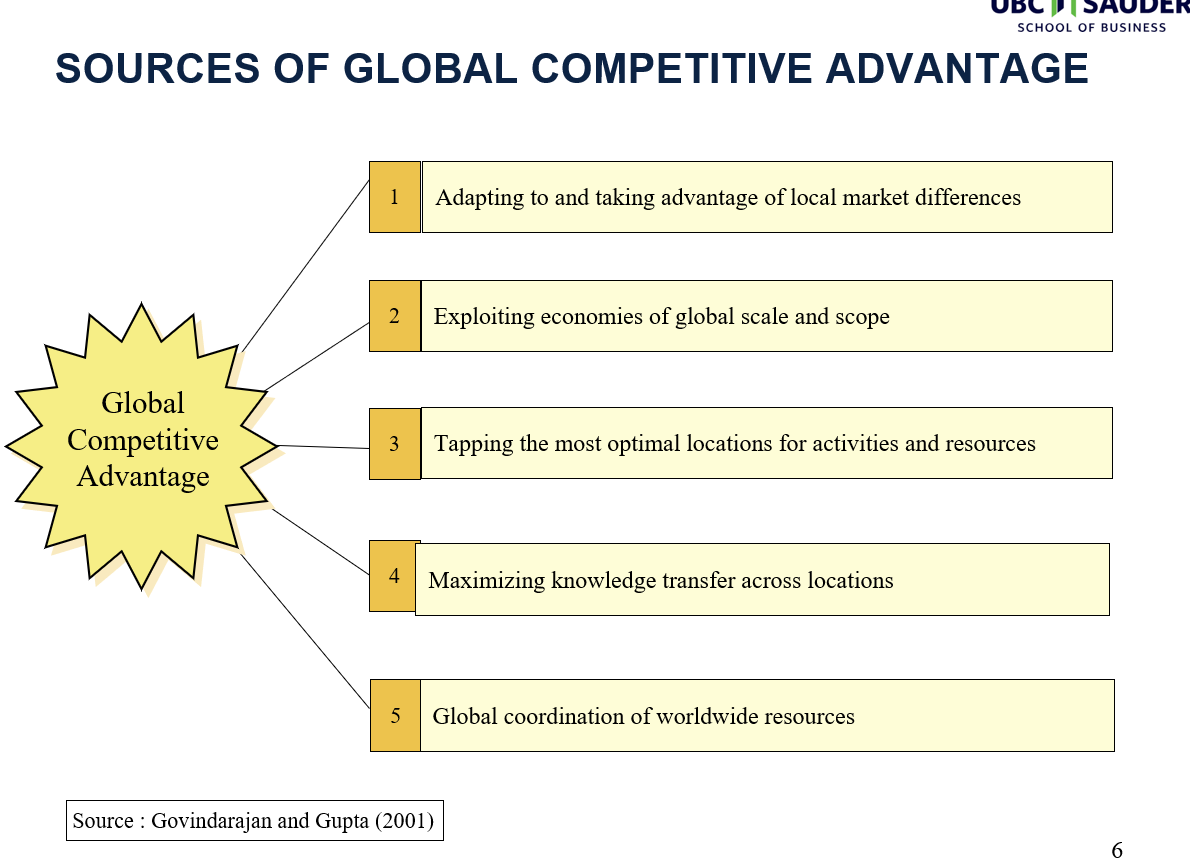
\includegraphics[width=0.8\linewidth,height=\textheight,keepaspectratio]{images/Screenshot 2025-08-02 013310.png}

}

\caption{\label{fig-old1}Original Screenshot 1}

\end{figure}%

\begin{figure}[H]

\centering{

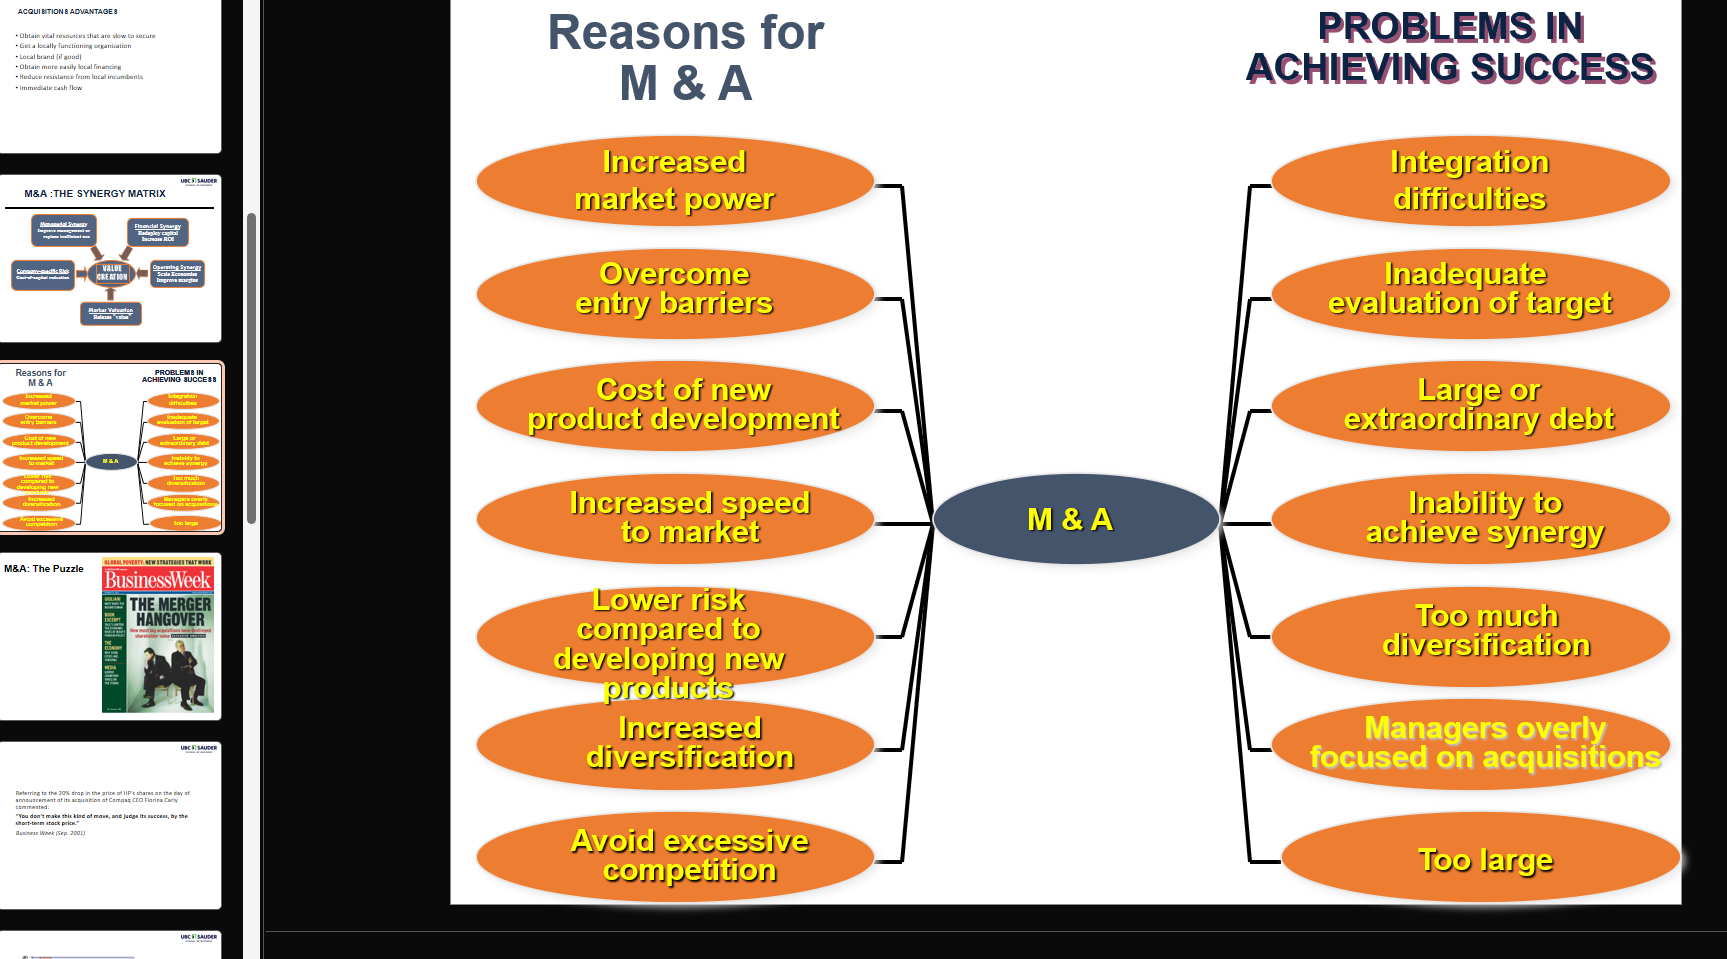
\includegraphics[width=0.8\linewidth,height=\textheight,keepaspectratio]{images/Screenshot 2025-08-02 021857.png}

}

\caption{\label{fig-old2}Original Screenshot 2}

\end{figure}%

\subsection{Updated Graphics}\label{updated-graphics}

\begin{figure}[H]

\centering{

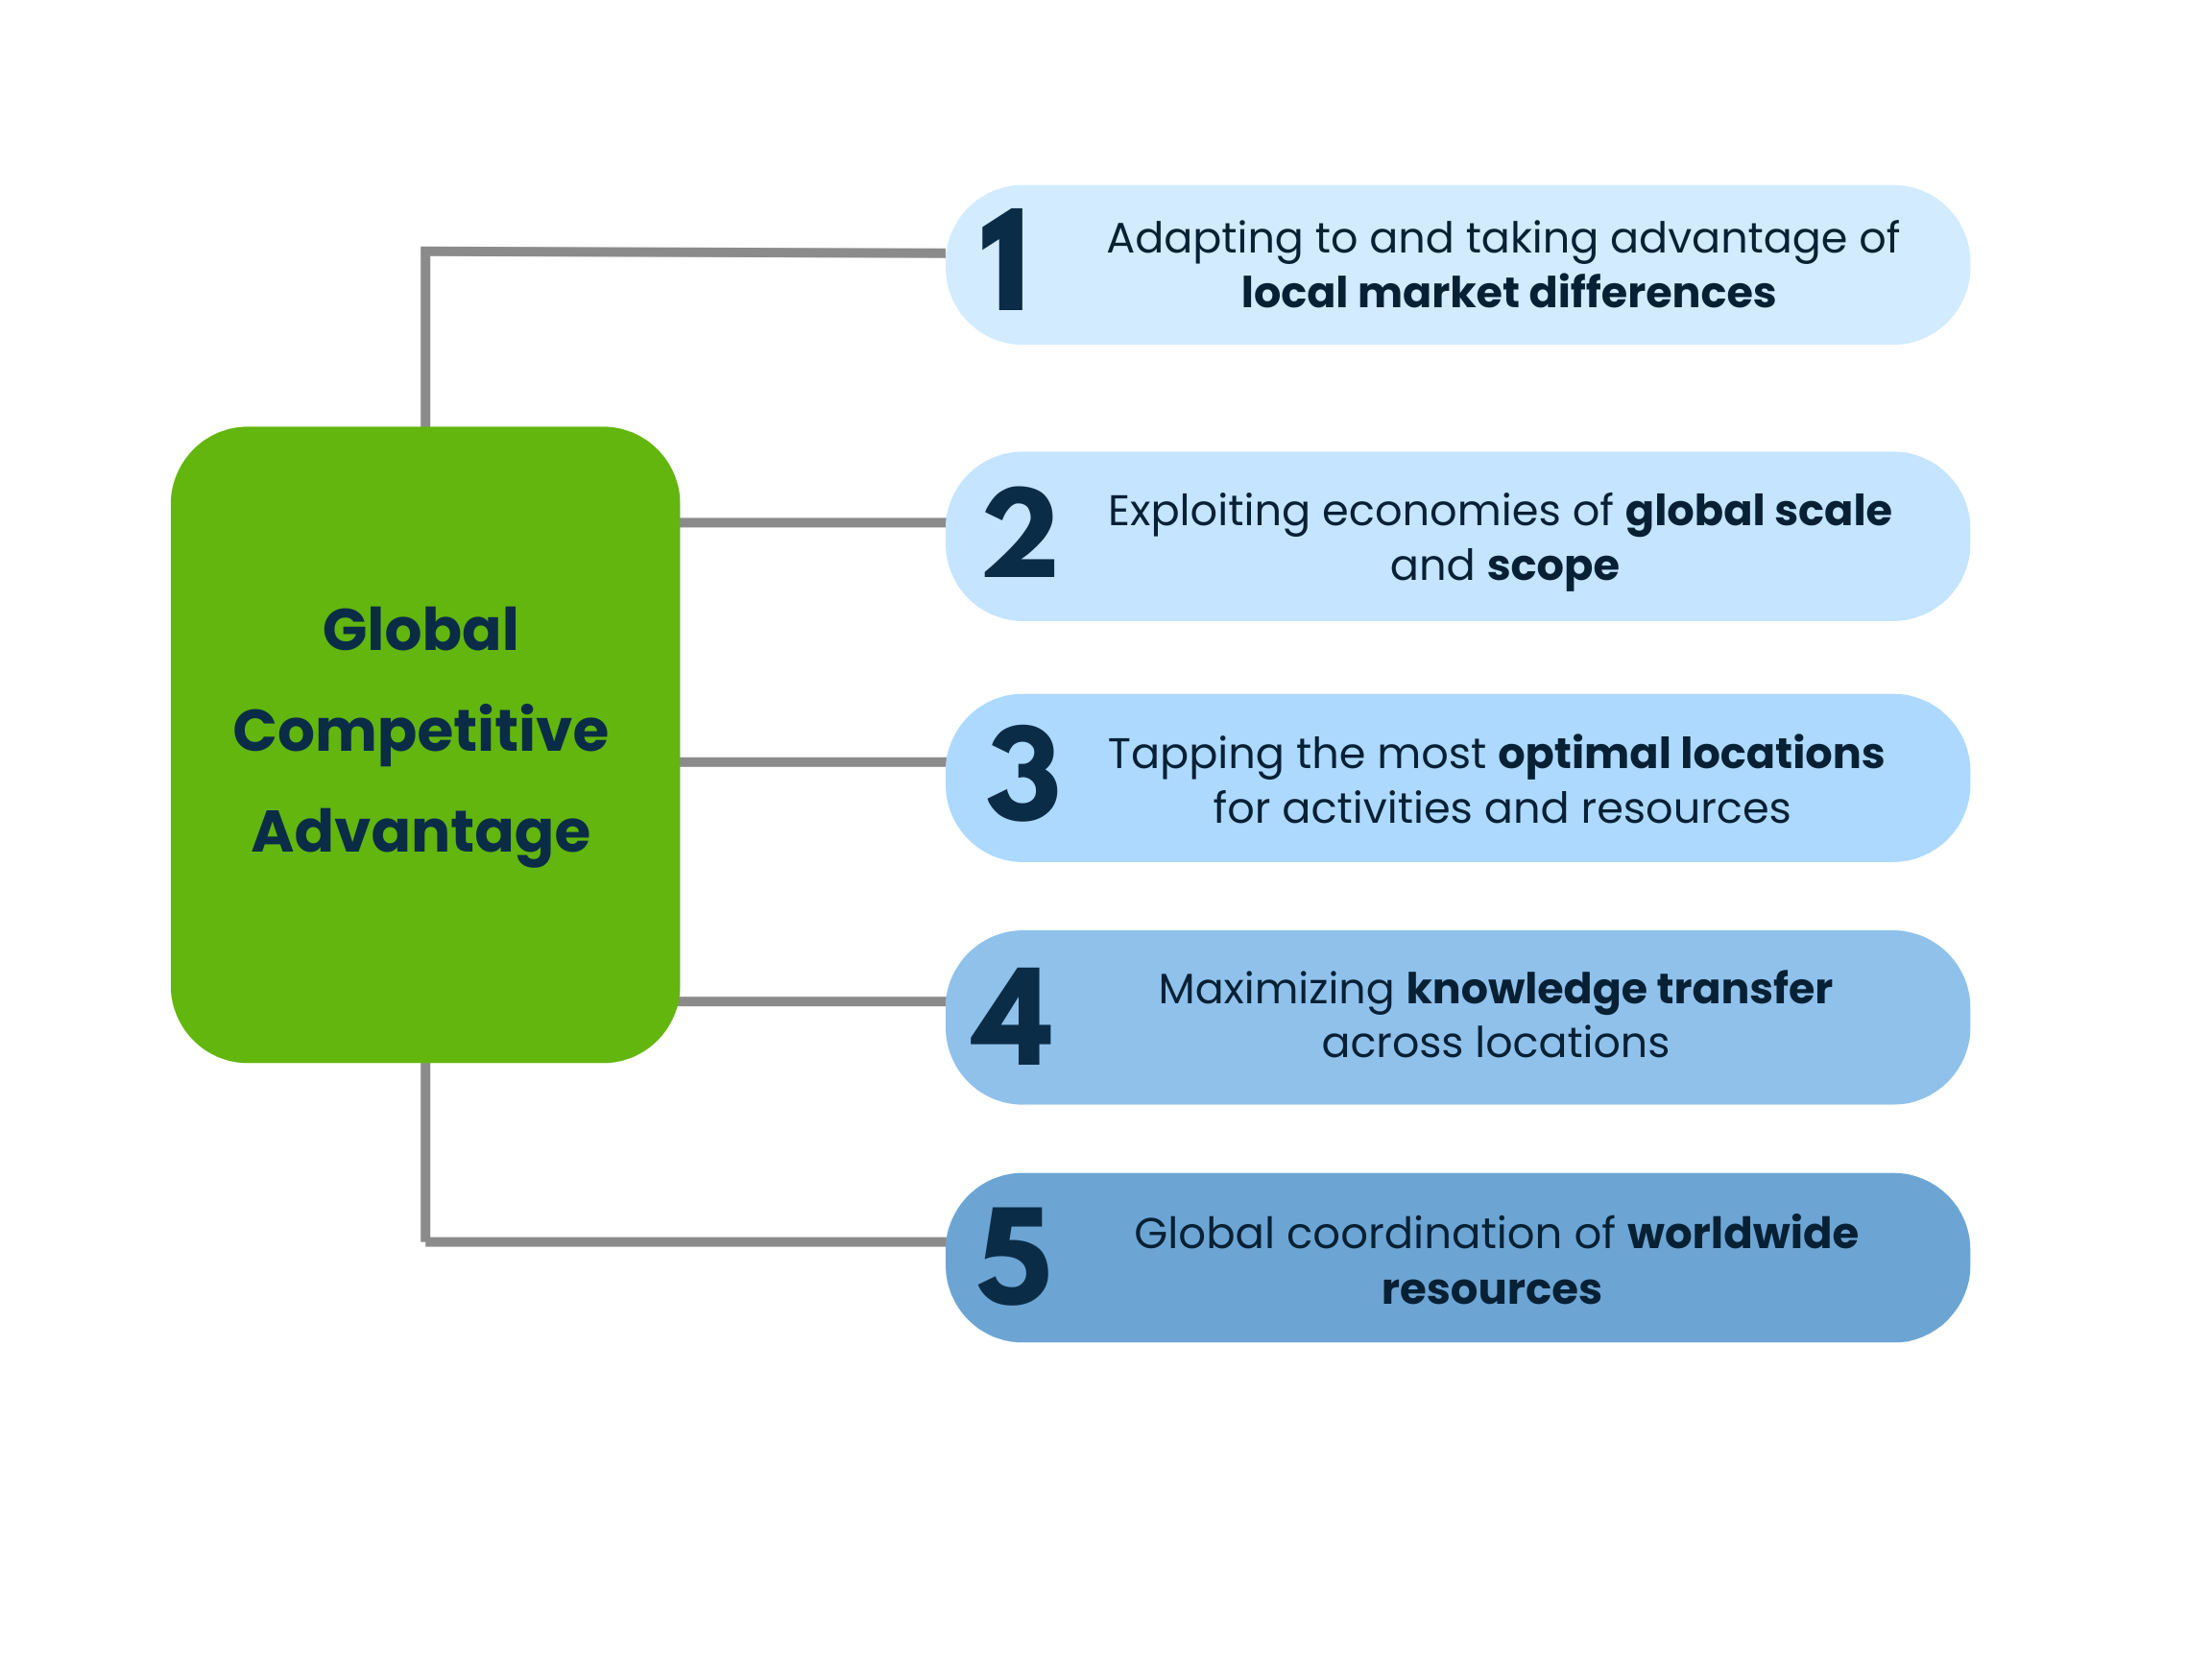
\includegraphics[width=0.8\linewidth,height=\textheight,keepaspectratio]{images/Updated_Images/1.png}

}

\caption{\label{fig-new1}Updated Graphic 1}

\end{figure}%

\begin{figure}[H]

\centering{

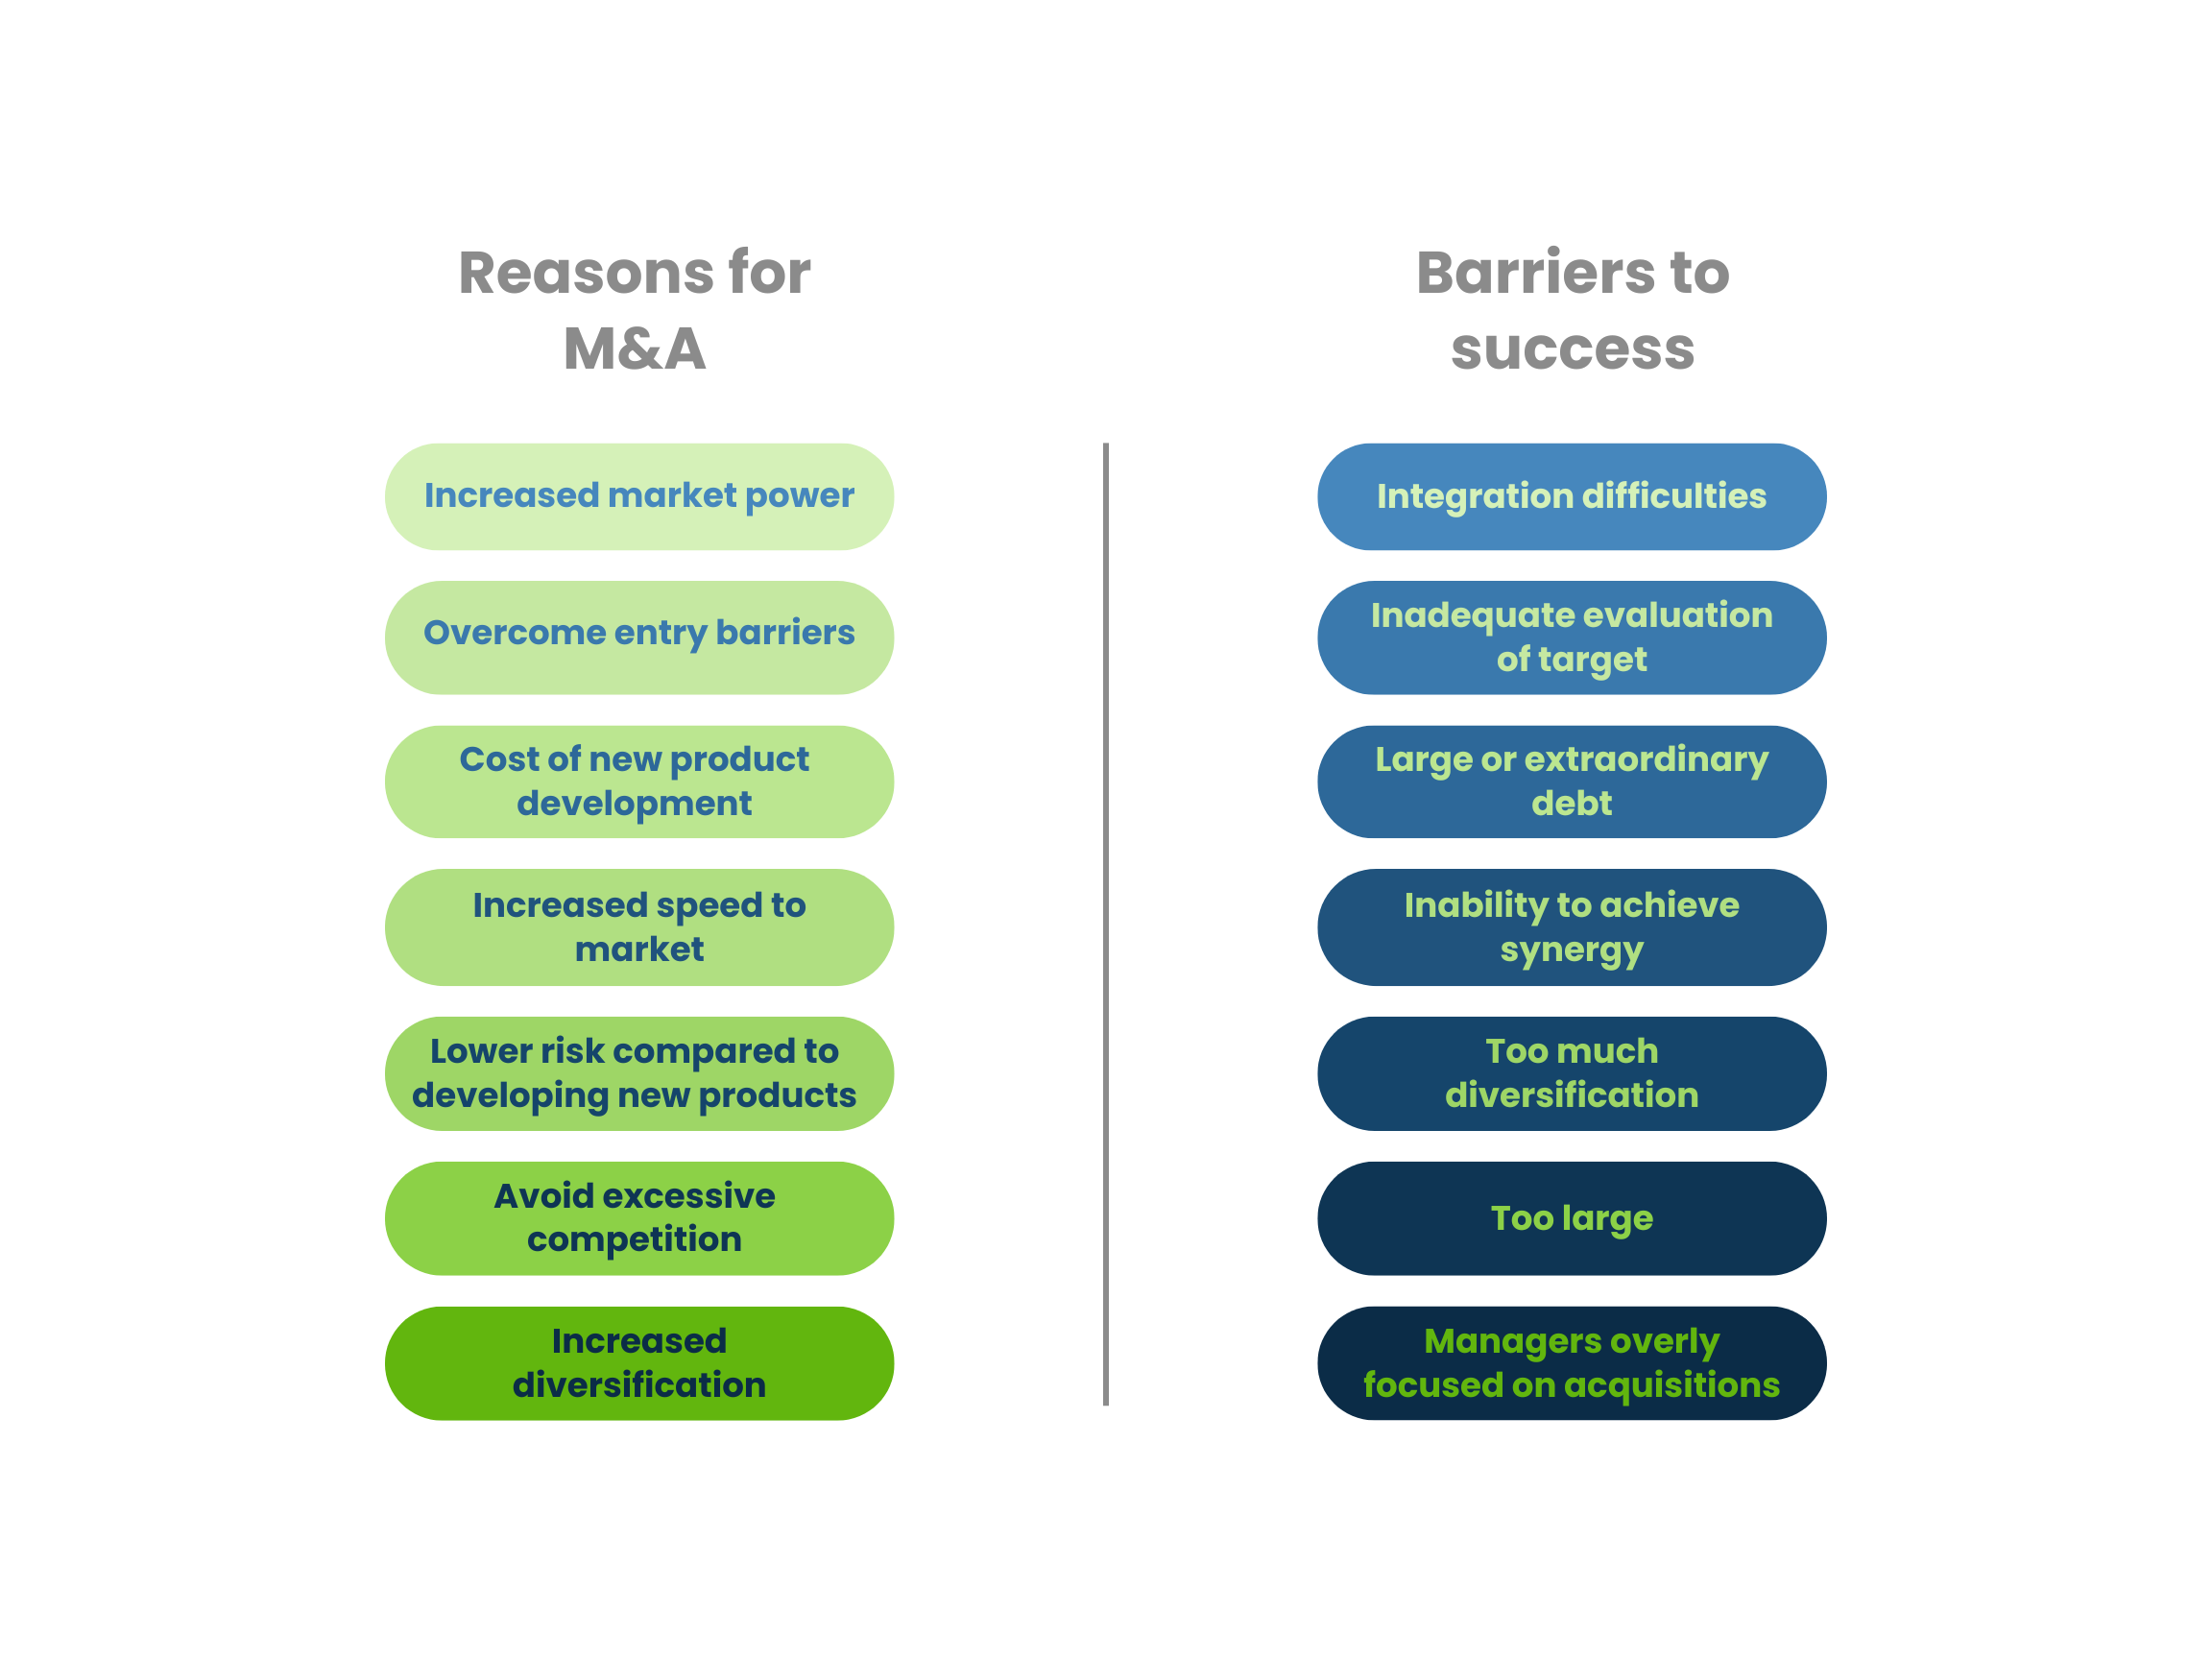
\includegraphics[width=0.8\linewidth,height=\textheight,keepaspectratio]{images/Updated_Images/2.png}

}

\caption{\label{fig-new2}Updated Graphic 2}

\end{figure}%

The updated graphics (Figure~\ref{fig-new1} and Figure~\ref{fig-new2})
provide improved visual clarity and enhanced presentation compared to
the original versions (Figure~\ref{fig-old1} and Figure~\ref{fig-old2}).

\section{Exercise Recommendations}\label{exercise-recommendations}

\subsection{Class 2: Globalization}\label{class-2-globalization}

\subsubsection{End-of-class exercise
question}\label{end-of-class-exercise-question}

\begin{itemize}
\tightlist
\item
  Given the benefits of globalization, why is ``slowbalization''
  occurring?
\end{itemize}

\subsubsection{International crisis response simulation
(Camille)}\label{international-crisis-response-simulation-camille}

To apply strategic thinking under uncertainty and crisis shocks in
international business, students will engage in a role-play scenario
where groups of students will assume the roles of executives and plan
their course of action.

\begin{itemize}
\tightlist
\item
  Group 1: CEO
\item
  Group 2: Regional Director
\item
  Group 3: Global Financial Manager
\item
  Group 4: International Business Development Manager
\end{itemize}

Objective: In groups of 3-4, students will analyze a case in which their
business is under threat from a global crisis (supply chain or
finance-related). They will then design a plan to mitigate the impacts
of this issue and maintain international operations, aligning with their
respective executive role. This exercise will encourage students to
critically examine globalization and the essential connections that
underpin it.

Scenario example: Your company is a mid-sized European retail brand
expanding aggressively into Southeast Asia, Latin America, and Africa.
You rely on an AI-based global logistics platform headquartered in
Singapore to manage inventory flows, delivery coordination, and supplier
tracking.

Overnight, the system is compromised by a malware attack traced to a
state-linked hacking group in Russia. Your AI platform is frozen,
shipments are delayed, and customer data may be exposed. The breach puts
your company's supply chain, public image, and financial stability at
risk.

Simulation Flow:

\begin{enumerate}
\def\labelenumi{\arabic{enumi}.}
\tightlist
\item
  10 minutes - Read the scenario and discuss within your group
\item
  15 minutes - Develop a strategic response from your role's perspective
\item
  5 minutes per group - Present your proposed response to the class
\item
  Class-wide debrief - Reflect on alignment/conflict between roles and
  real-world relevance
\end{enumerate}

\subsection{Class 3: Slowbalization}\label{class-3-slowbalization}

\subsubsection{End-of-class exercise
question:}\label{end-of-class-exercise-question-1}

\begin{itemize}
\tightlist
\item
  What is your prediction for the global economy in light of
  slowbalization? Will it continue or reverse? Explain your reasoning.
\end{itemize}

\subsection{Class 5: Gains and Costs from
Trade}\label{class-5-gains-and-costs-from-trade}

Turn international market analysis into a competitive activity where
teams act as firms choosing where to expand. Each country option has
different risk-reward profiles (tariffs, cultural barriers, supply chain
complexity), and teams justify their choices. Makes theoretical
frameworks more tangible. Acts as a low-stakes preliminary activity for
final project; gets students acquainted with this, may assist them in
ideation or execution of this project.

\subsubsection{Cross-National Trade Simulation
Activity}\label{cross-national-trade-simulation-activity}

To explore international trade and comparative advantage hands-on,
students will work in small groups, each representing a different
country.

\begin{itemize}
\tightlist
\item
  Group 1: United States\\
\item
  Group 2: China\\
\item
  Group 3: Germany\\
\item
  Group 4: Brazil
\end{itemize}

Objective: Using production data for two goods (e.g.~cars and bananas),
each group will:

\begin{enumerate}
\def\labelenumi{\arabic{enumi}.}
\tightlist
\item
  Calculate their opportunity cost for producing each good.
\item
  Identify their country's comparative advantage based on opportunity
  cost.
\item
  Negotiate trade agreements with other countries to maximize mutual
  benefits using knowledge gained from the course material
\item
  Strategically specialize in the good they produce most efficiently.
\item
  Achieve the highest combined total output via smart specialization and
  trade.
\end{enumerate}

\begin{quote}
This is a \textbf{timed competition:} the group that secures the most
advantageous trade deals and maximizes net gains from trade will be
recognized as the top global trading nation.
\end{quote}

Guidelines: - Use basic economic concepts (comparative advantage,
opportunity cost, specialization, gains from trade) - Each trade must be
recorded, including what was traded, with whom, and under what terms -
You must be able to explain the rationale for your decisions and how
opportunity costs informed your strategy

Example: One team represents USA and the other Brazil

\begin{longtable}[]{@{}lll@{}}
\toprule\noalign{}
Country & Cars & Bananas \\
\midrule\noalign{}
\endhead
\bottomrule\noalign{}
\endlastfoot
USA & 10 & 20 \\
Brazil & 5 & 25 \\
\end{longtable}

To determine the winner:

\begin{enumerate}
\def\labelenumi{\arabic{enumi}.}
\tightlist
\item
  Track all trades: Each group must keep a clear record of:

  \begin{itemize}
  \tightlist
  \item
    Goods produced
  \item
    Goods traded (and with whom)
  \item
    Goods consumed after trade
  \end{itemize}
\item
  Calculate total benefit:

  \begin{itemize}
  \tightlist
  \item
    Assign each good a value (e.g., Cars = 10 units, Bananas = 5 units)
  \item
    Sum the total value of the goods each country ends up with
    post-trade
  \item
    Assign a value to each good: Class can agree on a simple point
    system. For example:
  \end{itemize}
\end{enumerate}

1 Car = 10 points\\
1 Banana = 5 points

Now multiply:

USA's total value = (7 Cars × 10) + (15 Bananas × 5) = 70 + 75 = 145
points (if they chose to trade 3 cars)\\
Brazil's total value = (3 Cars × 10) + (10 Bananas × 5) = 30 + 50 = 80
points (if they chose to trade 15 bananas)

\begin{enumerate}
\def\labelenumi{\arabic{enumi}.}
\setcounter{enumi}{2}
\tightlist
\item
  Subtract opportunity costs:

  \begin{itemize}
  \tightlist
  \item
    Use your group's production data to estimate how many units of the
    other good you gave up (opportunity cost) when producing
  \item
    Deduct this from your final value to calculate net benefit (Net
    Benefit = Final Goods Value -- Opportunity Cost Value)
  \end{itemize}
\end{enumerate}

\subsection{Class 4/6/16/23 Current Threats to Globalization/Trade
Institutions/Global \& Regional
Strategies/Exercise}\label{class-461623-current-threats-to-globalizationtrade-institutionsglobal-regional-strategiesexercise}

\begin{itemize}
\tightlist
\item
  Already contains sufficient exercises
\end{itemize}

\subsection{Class 8/9 Plans for Internationalization/Location
Decision}\label{class-89-plans-for-internationalizationlocation-decision}

\begin{itemize}
\tightlist
\item
  Add exercises on Ghemawat's CAGE Framework
\item
  Add exercises on Location Grid Evaluation
\end{itemize}

\subsection{Class 11/12 Export and
Licensing}\label{class-1112-export-and-licensing}

You are company XYZ considering expanding but now you have to decide
whether to export or license????

\subsection{Class 13/14 FDI \& M\&A}\label{class-1314-fdi-ma}

\subsubsection{End-of-class exercise
question}\label{end-of-class-exercise-question-2}

Could Daimler Chrysler failures be avoided? How so? What are your
recommendations?

\subsection{Class 17: Technology
Disruption}\label{class-17-technology-disruption}

\subsubsection{AI and Globalization Simulation Activity
(Camille)}\label{ai-and-globalization-simulation-activity-camille}

To explore how artificial intelligence (AI) influences globalization,
students will work in small groups, each representing a distinct domain,
sector, or industry affected by AI in the global economy.

Group Assignments: - Group 1: Supply Chain and Logistics - Group 2:
Finance and Banking - Group 3: Manufacturing and Automation

Objective: Using real-world examples and economic concepts discussed in
class, each group will:

\begin{enumerate}
\def\labelenumi{\arabic{enumi}.}
\tightlist
\item
  Investigate how AI is transforming their assigned sector on a global
  scale.
\item
  Identify 2--3 key ways AI has influenced labor, trade, or innovation
  across country borders
\item
  Present a short ``case'' or simulated scenario that demonstrates how
  AI drives globalization in their sector.
\item
  Explain the geopolitical, ethical, and economic implications of these
  changes.
\item
  Compare AI's impact across sectors in a class-wide discussion on
  convergence/divergence in global outcomes.
\end{enumerate}

To Determine the Most Effective Group:

\begin{enumerate}
\def\labelenumi{\arabic{enumi}.}
\tightlist
\item
  \textbf{Content Depth}

  \begin{itemize}
  \tightlist
  \item
    Did the group provide specific, well-researched examples?
  \item
    Were connections to globalization clearly made?
  \end{itemize}
\item
  \textbf{Application of Course Concepts}

  \begin{itemize}
  \tightlist
  \item
    Did the group reference key ideas such as technological diffusion,
    labor shifts, or ethical challenges?
  \end{itemize}
\item
  \textbf{Creativity and Clarity}

  \begin{itemize}
  \tightlist
  \item
    Was the scenario engaging and easy to follow?
  \item
    Did the group make the topic relevant to real-world IB challenges?
  \end{itemize}
\item
  \textbf{Discussion Facilitation}

  \begin{itemize}
  \tightlist
  \item
    Did the group spark thoughtful discussion in the class-wide
    comparison?
  \end{itemize}
\end{enumerate}

\subsection{Class 19 Political Risk}\label{class-19-political-risk}

You are Mills Manufacturing, a local US North Carolina parachute factory
producing 5,000 parachutes a year, wherein a quarter of your workforce
are immigrants working under temporary legal protection. Recent
political developments have made it unfeasible for this quarter of your
workforce to continue working. You are the CEO of Mills Manufacturing
and need to make a decision. How will you cope with this sudden
political shift?

Relevant Links: -
\href{https://archive.ph/Sv9RA\#selection-2617.85-2617.256}{Only Two
Companies Make Parachutes for U.S. Troops. Deportations Would Crush One}
- \href{https://archive.ph/pp4xl}{ICE Raids} -
\href{https://www.theguardian.com/us-news/2025/jul/29/trump-immigration-crackdown-labor-shortages-slowdowns}{Guardian:
Trump Immigration Crackdown, Labor Shortages}

\subsection{Class 21/22 Cross Cultural
Management}\label{class-2122-cross-cultural-management}

Possible role play exercise: Suppose we are a Japanese firm
collaborating with a North American firm. What are the things we need to
keep in mind in order to have a successful collaboration.

\subsection{Class 24 Ethics}\label{class-24-ethics}

Managing cross-cultural ethical conflicts. Suppose you are President
Trump (POTUS) and need to manage trade conflict with Canada, Japan, and
Iran. Using what you have learned in class, what strategy would you
pursue.

\section{Final Project - International Expansion
Case}\label{final-project---international-expansion-case}

Objective: Apply strategic analysis tools to identify and solve a
company's core business challenges within an international context,
resulting in a recommendation that addresses both firm-specific and
global market dynamics

\subsubsection{Notes \& suggestions:}\label{notes-suggestions}

\begin{itemize}
\tightlist
\item
  Rubric could include a section on presentation of case report (e.g.,
  visuals, organization of information, logical flow of report).
\item
  Could include contingency analysis: missing a risk assessment and plan
  to mitigate potential challenges.
\item
  Important to consider how implementation would vary under conditions
  of different nations (political situation, tastes, social \& economic
  factors)
\end{itemize}


\printbibliography



\end{document}
